\begin{kbox}{6. 窄带随机过程 (核心结论)}
    \textbf{定义}:带宽 $\Delta f \ll f_c$ 且远离零频的随机过程。
    
    \tcbline
    
    \begin{minipage}{0.65\linewidth}
        \textbf{表达式}:
        \begin{itemize}
            \item \textbf{包络相位法}:
            \[ \xi(t) = a_{\xi}(t) \cos[\omega_c t + \phi_{\xi}(t)] \]
            \item \textbf{同相正交法}:
            \[ \xi(t) = \xi_c(t) \cos \omega_c t - \xi_s(t) \sin \omega_c t \]
        \end{itemize}
    \end{minipage}%
    \begin{minipage}{0.35\linewidth}
        \centering
        % 融入笔记中的矢量三角形
        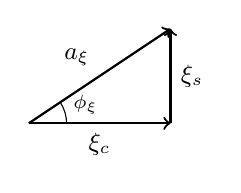
\begin{tikzpicture}[scale=1.2]
            \draw[thick, ->] (0,0) -- (1.5,0) node[midway, below] {\small $\xi_c$};
            \draw[thick, ->] (1.5,0) -- (1.5,1.0) node[midway, right] {\small $\xi_s$};
            \draw[thick, ->] (0,0) -- (1.5,1.0) node[midway, above left] {\small $a_\xi$};
            \draw (0.4,0) arc (0:33.69:0.4);
            \node at (0.6,0.2) {\scriptsize $\phi_\xi$};
        \end{tikzpicture}
    \end{minipage}

    \tcbline 
    
    \textbf{统计特性} (设 $\xi(t)$ 均值0,方差 $\sigma_{\xi}^2$):
    \begin{enumerate}
        \item $\xi_c(t), \xi_s(t)$ 均为高斯过程,均值0,方差 $\sigma_{\xi}^2$。
        \item \textbf{重要结论}:同一时刻,$\xi_c$ 与 $\xi_s$ \textbf{互不相关} (即统计独立)。
        \item \textbf{包络 $a_{\xi}$ (瑞利分布)}:$f(a_{\xi}) = \frac{a_{\xi}}{\sigma_{\xi}^2} e^{-\frac{a_{\xi}^2}{2\sigma_{\xi}^2}}, \ (a_{\xi} \geq 0)$
        \item \textbf{相位 $\phi_{\xi}$ (均匀分布)}:$f(\phi_{\xi}) = \frac{1}{2\pi}, \ (0 \leq \phi_{\xi} \leq 2\pi)$
    \end{enumerate}
\end{kbox}

\begin{kbox}{7. 白噪声与带限噪声}
    \textbf{基本概念}:
    \begin{itemize}
        \item \textbf{白噪声}:在整个频带内功率谱密度 (PSD) 都平坦的噪声。
        \item \textbf{高斯白噪声}:概率分布服从高斯分布,且 PSD 均匀的噪声。
        \item \textbf{带限白噪声}:白噪声通过有限带宽信道或滤波器后的噪声。
    \end{itemize}

    \tcbline

    \textbf{理想白噪声}:
    \begin{itemize}
        \item PSD (双边):$P_n(f) = n_0 / 2$
        \item 自相关:$R(\tau) = \frac{n_0}{2} \delta(\tau)$
    \end{itemize}
    
    \textbf{低通白噪声 (LPF, 截止 $f_H$)}:
    \[ R(\tau) = n_0 f_H \frac{\sin 2\pi f_H \tau}{2\pi f_H \tau} = n_0 f_H \operatorname{Sa}(2\pi f_H \tau) \] 
    
    \textbf{带通白噪声 (BPF, 带宽 $B$)}:
    \[ R(\tau) = n_0 B \frac{\sin \pi B \tau}{\pi B \tau} \cos 2\pi f_c \tau, \quad N = n_0 B \]
\end{kbox}

\begin{kbox}{8. 正弦波 + 窄带高斯噪声}
    \textbf{包络 $z$ 服从莱斯 (Rice) 分布}:
    \[ f(z) = \frac{z}{\sigma_n^2} \exp\left[-\frac{z^2 + A^2}{2\sigma_n^2}\right] I_0\left(\frac{Az}{\sigma_n^2}\right) \]
    ($A$: 信号振幅, $\sigma_n^2$: 噪声方差, $I_0$: 修正贝塞尔)
\end{kbox}